\begin{figure}

\centering
\code{c = \createlatch(2);}

\vspace{-12pt}
\[
\left(
\begin{tabular}{ 
  l@{\extracolsep{\fill}} || 
  l@{\extracolsep{\fill}} || 
  l@{\extracolsep{\fill}} }
\BCOMMENT{\SPEC{$T_1$}} & \BCOMMENT{\SPEC{$T_2$}} & \BCOMMENT{\SPEC{$T_3$}}\\
\code{h=hs*cosine($\theta$/2);} & 
\code{r=hs*sine($\theta$/2);} & \\
\code{countDown(c);} & \code{countDown(c);} & \code{await(c);}\\
& & \code{V=(1/3)*$\pi$*power(r,2)*h;}\\
\end{tabular}\!\!\right)%\!\!\code{;}
\]

\begin{tabular}{ll}
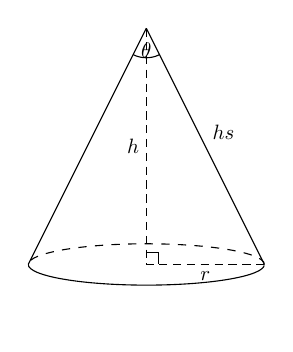
\begin{tikzpicture}[scale=0.75, every node/.style={transform shape}]
 \begin{scope}
   \clip (-2,0) rectangle (2,1cm);
   \draw[dashed] (0,0) circle (2cm and 0.35cm);
 \end{scope}
 \begin{scope}
   \clip (-2,0) rectangle (2,-1cm);
   \draw (0,0) circle (2cm and 0.35cm);
 \end{scope}
   \draw[densely dashed]
        (0,4) coordinate (c)
     -- node[auto=right] {$h$}            %,font=\footnotesize
        coordinate[pos=0.95] (aa) (0,0)
     -- node[below] {$r$} 
        coordinate[pos=0.1]  (bb) (2,0);
   \draw (aa) -| (bb);
   \draw (c) -- (-2,0) coordinate (a);
   \draw (c) -- node [auto=left] {$hs$} 
                (2,0) coordinate (b);
   \begin{scope}
     \path[clip] (a) -- (c) -- (b) -- cycle;
     \draw (c) circle (5mm) node [label=below:$\theta$]{};
   \end{scope}    
\end{tikzpicture}

&
\pause
\begin{tikzpicture}[every node/.style={anchor=base,
    text height=.8em,text depth=.2em,minimum size=7mm},
    ->, >=stealth']
    
  \matrix{
    \node[] (lbl) {\code{cnt=2}};\\
    %\node[fill=gray!30] (cnt_init) {$2$};\\
    \node[fill=gray!30,draw] (cnt_2) {$2$};\\
    \node[fill=gray!20,draw] (cnt_1) {$1$};\\
    \node[fill=gray!10,draw] (cnt_0) {$0$};\\
    \node[] (cnt_end) {};\\
  };
  
    \node[left= of cnt_2] (tm) {$T_3$};
    \node[left= of cnt_1] (t1) {$T_1$};
    \node[left= of cnt_0] (t2) {$T_2$};
  
    \node[right=15pt of cnt_2] (wait) {awaiting $\ldots$};
    \node[right=15pt of cnt_1] (cont_1) {$T_1$, continue};
    \node[right=15pt of cnt_0] (cont_2) {$T_2$, continue};
    \node[right=15pt of cnt_end] (cont_m) {$T_3$, resume};
  
  \path (tm) edge node [->, scale=.58, auto] {\code{await()}} (cnt_2);
  \path (t1) edge node [->, scale=.58, auto] {\code{countDown()}} (cnt_1);
  \path (t2) edge node [->, scale=.58, auto] {\code{countDown()}} (cnt_0);
  
  %\draw [->, dashed] (cnt_2) to node [] {} (wait);
  \draw [->, dashed] (cnt_1) -- node [] {} (cont_1);
  \draw [->, dashed] (cnt_0) -- node [] {} (cont_2);
  \draw [->, dashed, auto] (cnt_0) |- node [below] {\code{cnt=0}} (cont_m);
\end{tikzpicture}
\end{tabular}

\end{figure}
